\documentclass{article}
\usepackage[utf8]{inputenc}
\usepackage[margin=0.9in]{geometry}
\usepackage{titling}
\usepackage[utf8]{inputenc}
\usepackage[english]{babel}
\usepackage{amsthm}
\usepackage{amsmath}
\usepackage{amssymb}
\usepackage{graphicx}
\usepackage{changepage}

\graphicspath{ {/home/marko/Problem solving maths group} }
\newtheorem{theorem}{Theorem}
\newtheorem{definition}{Definition}
\newtheorem{example}{Example}
\newtheorem{exercise}{Exercise}

\title{\textbf{Discrete Geometry 1}\\Pick's Theorem}
\date{Week 2}
\author{Miroslav Stankovic\\ Marko Puza}
\begin{document}
\maketitle

\section*{Intro}

\emph{Discrete Geometry} is a branch of mathematics dealing with combinations and arrangements of geometric objects and discrete properties of such objects. Questions in discrete geometry usually involve countable sets of geometrical objects, such as points, lines, polygons and in general don't involve the notion of continuity. \\ Today, we will take a look at two different ways to calculate the area of simple\footnote{A polygon is simple if its sides don't intersect.} polygons. First, we will deduce one of the most significant theorems in the area of Discrete geometry - the Pick's Theorem. This will be followed by introducing the Shoelace formula and a small discussion about how useful these theorems are.


\section*{Pick's Theorem}

The theorem deals with geometry on a grid of equal-distanced points (i.e., points with integer coordinates). It states that the area $A$ of a simple polygon with vertices in the grid points can be found as:
 \[A = i + \frac{b}{2} - 1\] where $i$ is the number of grid points in the interior of the polygon and $b$ the number of grid points on the polygon boundary. \\

\begin{center}
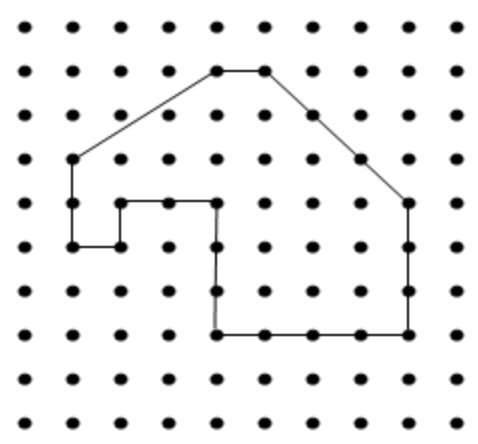
\includegraphics[width=4cm]{pick}
\end{center}

\begin{exercise}
	Show that the formula holds for all rectangles.
\end{exercise}

\begin{exercise}
	Show that the formula holds for all right-angled triangles.
\end{exercise}

\begin{exercise}
	Show that the formula holds for all triangles.
\end{exercise}

\begin{exercise}
	Show that if the formula holds for two polygons which share a segment of their perimeter, it also holds for the union of the two.
\end{exercise}

\begin{exercise}[Pick's Theorem]
	Show that for any simple polygon:  $A = i + \frac{b}{2} - 1$.
\end{exercise}

\begin{exercise}
	Consider a grid with unit-length between two points equal to $\sqrt{2}$. Show that every simple polygon with vertices in grid points has an integral area.
\end{exercise}

\begin{exercise}
	Does the formula change for polygons with holes?
\end{exercise}

\begin{exercise}
	Can the theory be extended to more dimensions?
\end{exercise}

\begin{exercise}
    Is there a similar formula for triangular grids?
\end{exercise}

\section*{Shoelace formula}
The Shoelace formula provides a way to compute the area of any simple polygon given the coordinates of all vertices. Suppose we have a simple polygon with $n$ sides and vertices $(x_i, y_i); \ i = 1, \dots, n$. Then its area $A$ is: \[A = \frac{1}{2} |(x_1 y_2 + x_2 y_3 + \cdots + x_{n-1} y_n + x_n y_1)  - (x_2 y_1 + x_3 y_2 + \cdots + x_n y_{n-1} + x_1 y_n)|\]
or, equivalently:
\[A = \frac{1}{2}|\sum_{i=1}^n \det{\left( \begin{smallmatrix} x_i&x_{i+1}\\ y_i&y_{i+1} \end{smallmatrix} \right)}|\]
where $x_{n+1} = x_1, y_{n+1} = y_1$. \\\\
Where does the name of the formula come from? Let's try to use the formula on a trianlge with vertices in points $(2, 4), (3, -8), (1, 2)$. This gives us: $A = \frac{1}{2} | (2 \cdot (-8) + 3 \cdot 2 + 1 \cdot 4) - (4 \cdot 3 + (-8) \cdot 1 + 2 \cdot 2) | = 7$.

\begin{center}
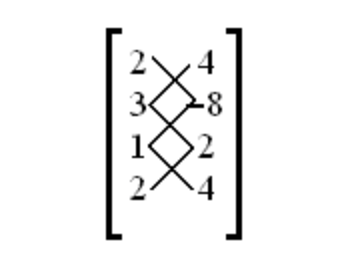
\includegraphics[width=4cm]{shoelace}
\end{center}

\begin{exercise}
    Show that the shoelace formula holds for any triangle.
\end{exercise}

\begin{exercise}
    Use this to prove that the shoelace formula holds for any convex polygon.
\end{exercise}

\begin{exercise}
Most of the time, the computer programs estimate all shapes by polygons - thus both Pick's theorem and the Shoelace formula could be applied to estimate their areas. Can you think of simple algorithms for both? What is their efficiency?
\end{exercise}

\begin{exercise}
Given $n$ vertices of a simple polygon, devise an $\mathcal{O}(n)$ algorithm to find the number of integer points that are inside the polygon or on its boundary.
\end{exercise}

\end{document}
